\documentclass[tikz,border=10pt]{standalone}
% Scale: s = 0.018182 cm per px, origin at ink-bbox centre (244, 192.5), y flipped
\begin{document}
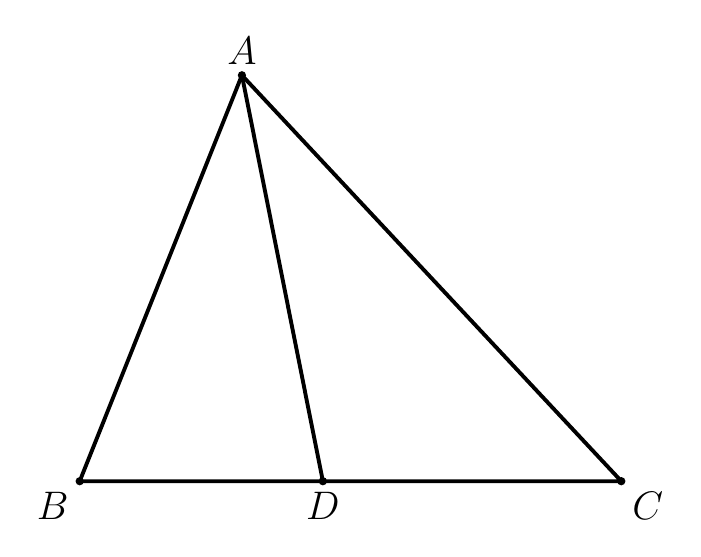
\begin{tikzpicture}[line width=1.4pt, line join=round]
  % Named coordinates (converted from image pixels)
  \coordinate (A) at (-1.384, 2.564);
  \coordinate (B) at (-3.444, -2.591);
  \coordinate (C) at ( 3.434, -2.591);
  \coordinate (D) at (-0.356, -2.591);

  % Triangle ABC, solid black
  \draw (A) -- (B) -- (C) -- cycle;

  % Cevian AD (not a right angle, no marker)
  \draw (A) -- (D);

  % Vertex dots
  \fill (A) circle (1.5pt);
  \fill (B) circle (1.5pt);
  \fill (C) circle (1.5pt);
  \fill (D) circle (1.5pt);

  % Labels in math mode, sized from style metrics
  \node[above, font=\fontsize{15}{18}\selectfont] at (A) {$A$};
  \node[below left, font=\fontsize{15}{18}\selectfont] at (B) {$B$};
  \node[below right, font=\fontsize{15}{18}\selectfont] at (C) {$C$};
  \node[below, font=\fontsize{15}{18}\selectfont] at (D) {$D$};
\end{tikzpicture}
\end{document}